%*******************************************************************************
%*********************************** Chapter XXXXXXXX *****************************
%*******************************************************************************
\chapter{The Deep Underground Neutrino Experiment}  %Title of chapter

\graphicspath{{DUNE/Figs/PDF/}{DUNE/Figs/Raster/}{DUNE/Figs/Vector}}

\nomenclature[a-tick]{tick}{Unit of time equal to 500 ns}
\nomenclature[z-CRC]{CRC}{Cosmic Ray Counter}
\nomenclature[z-SiPM]{ADC}{Analogue to Digital Converter}
\nomenclature[z-TPC]{TPC}{Time Projection Chamber}
\nomenclature[z-SiPM]{SiPM}{Silicon Photo Multiplier}
\nomenclature[z-CRC]{SSP}{SiPM Signal Processor}

%********************************** %First Section  **************************************
\section{DUNE location and beamline} %Section - X.1 

%********************************** %Second Section  *************************************
\section{The DUNE detectors and schedule} \label{sec:DUNEDetector} %Section - X.2

%********************************** %Third Section  *************************************
\section{Physics opportunities of DUNE} %Section - X.3

%********************************** % 3.1 Section  *************************************
\subsection{Neutrino physics}  %Section - X.3.1

%********************************** % 3.2 Section  *************************************
\subsection{Nucleon decay and supernovae neutrinos}  %Section - X.3.2

%********************************** % Fourth Section  *************************************
\section{Path to building DUNE - The 35 ton prototype} \label{sec:The35tonDetector}  %Section - X.4

\begin{figure}[h]
  \centering
  %\includegraphics[width=0.85\textwidth]{}
  \caption[The wrapped wires of the 35 ton]{A schematic showing what the wrapped wire planes of the DUNE detector designs looked like in the 35 ton.}
  \label{fig:35tonWireGeom}
\end{figure}

%********************************** % Fifth Section  *************************************
\section{The DUNE software} \label{sec:LArSoft} %Section - X.5
The software packed used by DUNE is called LArSoft~\citep{Church_LArSoft} which is a simulation, reconstruction and analysis package for LArTPCs which is being used by many of the experiments in the US neutrino program. LArSoft has been developed to be detector agnostic, meaning that much of the code is shared between experiments. To this end it is envisioned that it will be used as a platform for constant development in both existing experiments and those still in the planning phases such as DUNE. LArSoft is built around the Fermilab-supported analysis reconstruction framework (\emph{art}). External packages such as ROOT~\citep{ROOT} and GEANT4~\citep{GEANT4} are incorporated into LArSoft meaning that the user does not have to co-ordinate specific versions of the packages as the newest versions are automatically incorporated. \\

There are numerous mechanisms by which particles can be generated within the software with external packages such as GENIE~\citep{GENIE}, Nuance~\citep{Nuance} and CRY~\citep{CRY} already having been incorporated. Recently the MUon Simulations UNderground (MUSUN)~\citep{MUSUN} generator which takes the output of MUon SImulation Code (MUSIC)~\citep{MUSIC} has also been incorporated, see Section~\ref{sec:FDIncorporation}. It is also possible to use an inbuilt single particle generation mode which is fully tunable as particle type, momenta, positions and directions can all be varied. \\

The co-ordinates and angles in LArSoft, shown in Figure~\ref{fig:LArSoft_coords}, are defined as;
\begin{itemize}
\item $x$ - The beam direction, with maximal $x$ being where the beam enters the detector.
  \begin{itemize}
  \item In the 35 ton prototype where there is no beam positive x is in the opposite direction to that which electrons drift in the large TPC where $x$ = 0 is the position of the APA frames in the long drift volume.
  \item In the far detector geometry $x$ = 0 is defined as .......
  \end{itemize}
\item $y$ - The vertical direction, with maximal $y$ being the most highest point.
  \begin{itemize}
  \item In the 35 ton $y$ = 0 is halfway between the gap created by the two centre APAs which are mounted one above the other.
  \item In the far detector $y$ = 0 is .........
  \end {itemize}
\item $z$ - Defined as such to have a right handed co-ordinate system.
  \begin{itemize}
  \item In the 35 ton $z$ = 0 is at the edge of the leftmost APA frame when looking down the long drift volume.
  \item In the far detector $z$ = 0 is .........
  \end{itemize}
\item $\theta$ - The angle that a point makes from the $x$ axis in the $xy$ plane.
\item $\phi$ - The angle between the $z$ axis and the point.
\end{itemize}

\begin{figure}[h]
  \centering
  \begin{subfigure}{0.45\textwidth}
    \centering
    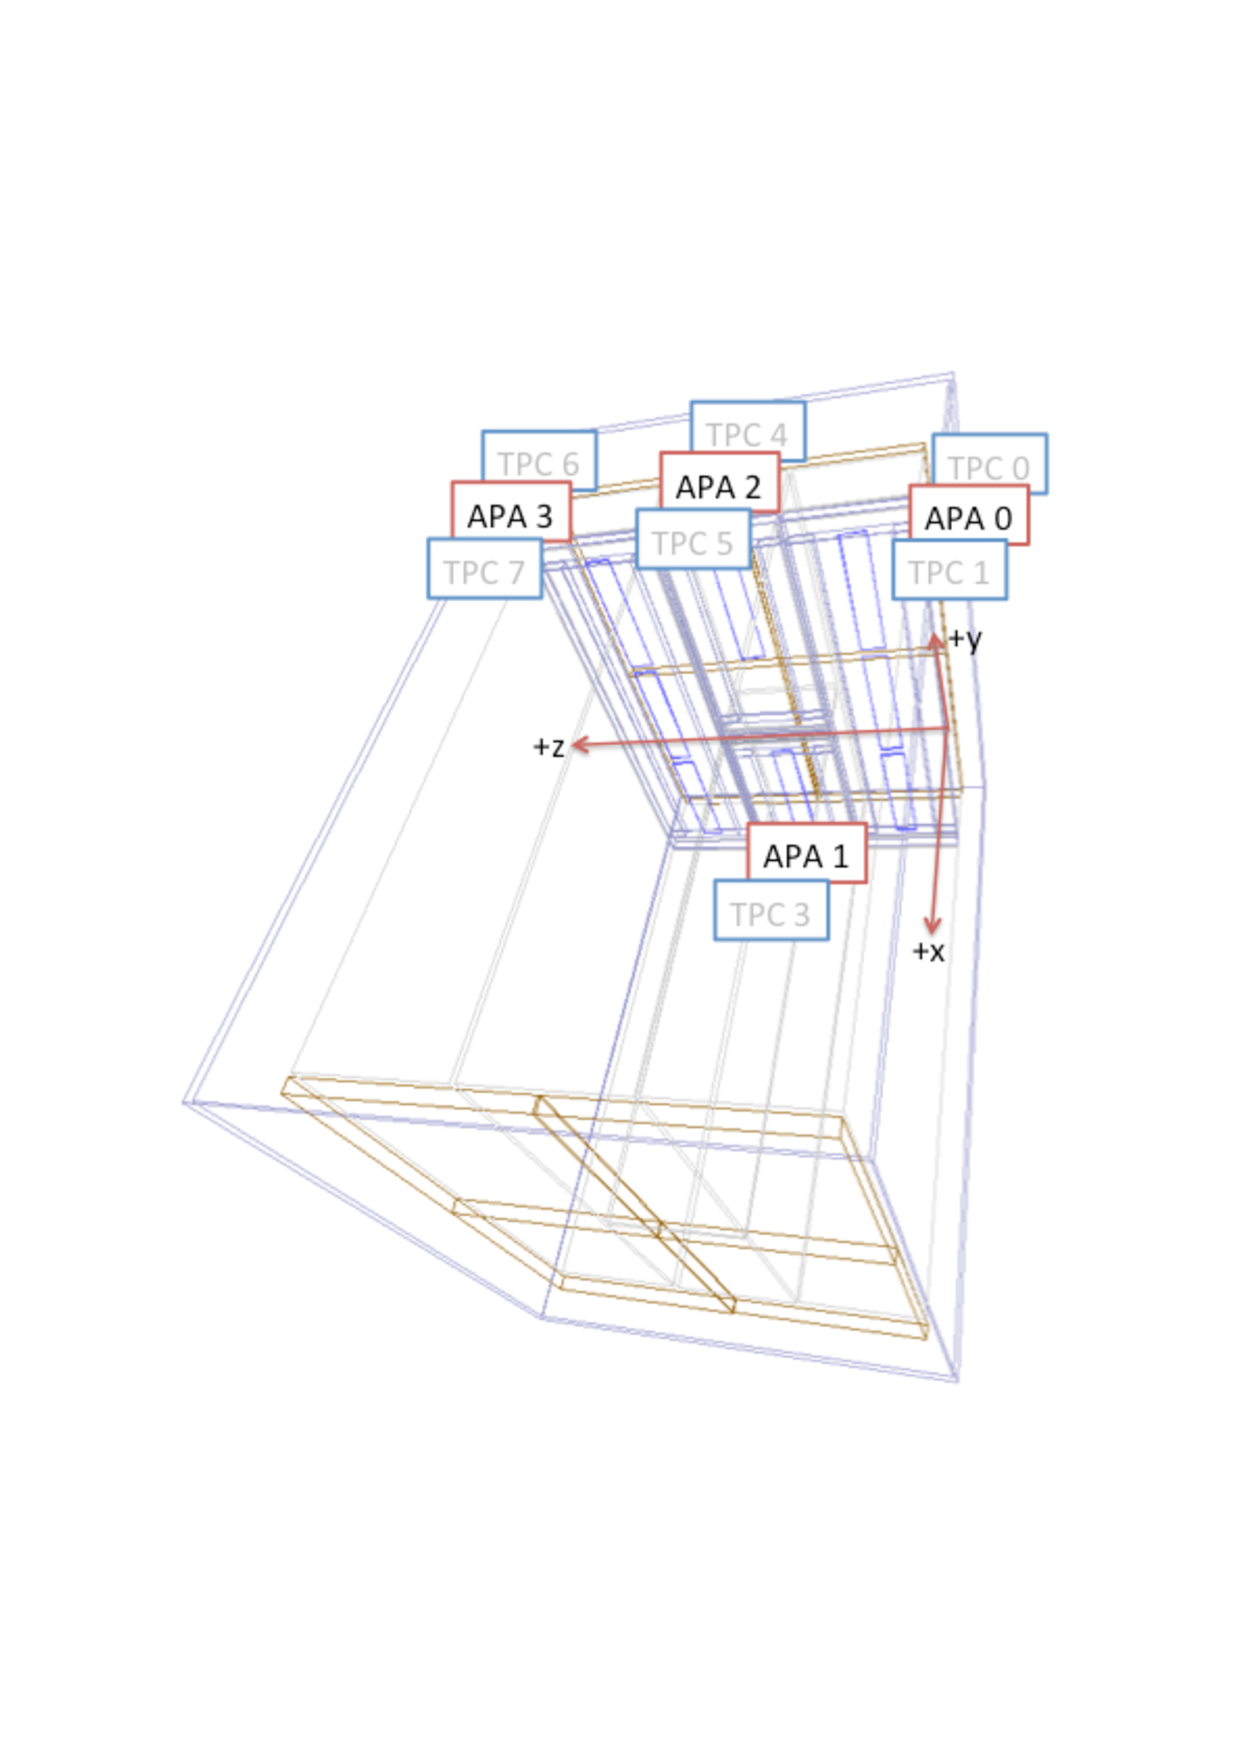
\includegraphics[width=\textwidth]{35ton_APASchem}
    \caption{The location of the origin of the 35 ton co-ordinate system in 3D.}
  \end{subfigure}
  \hspace{0.08\textwidth}
  \begin{subfigure}{0.45\textwidth}
    \centering
    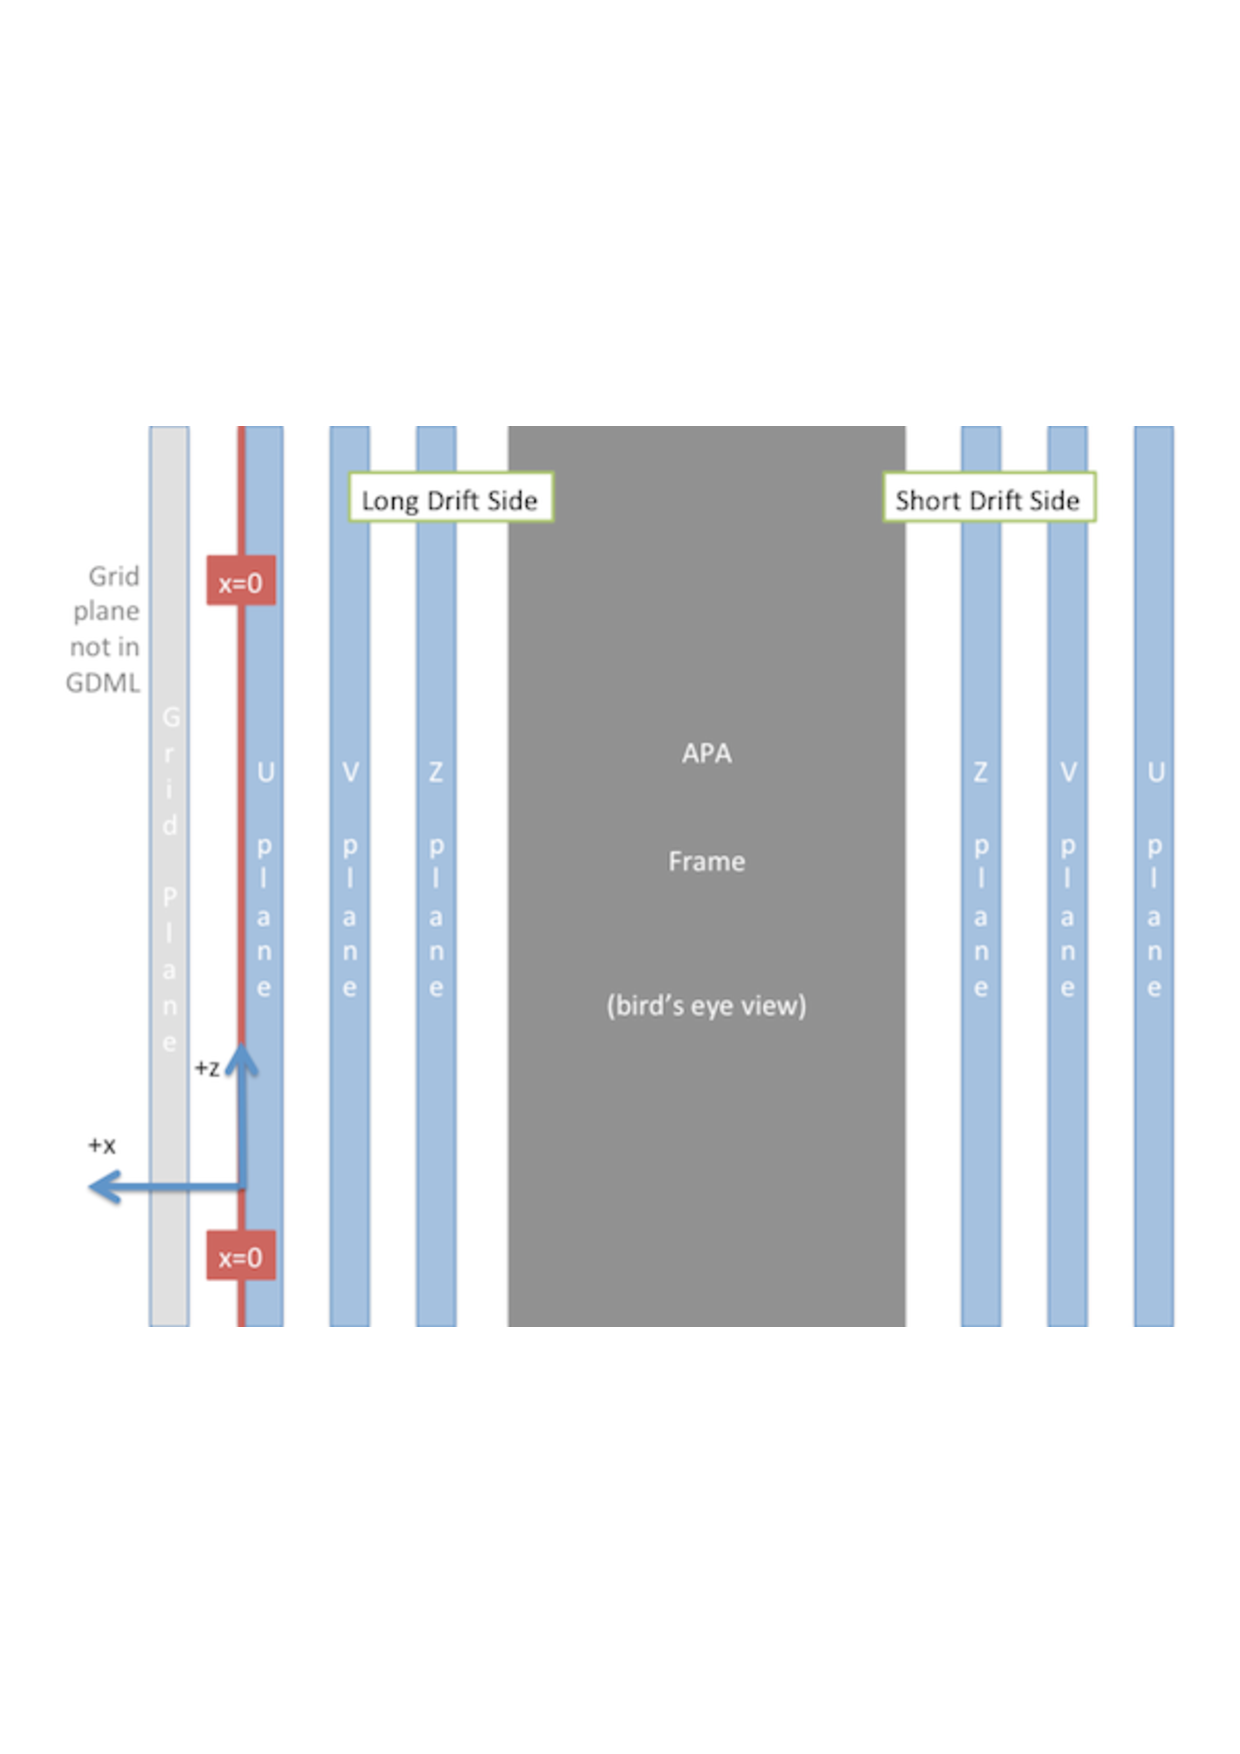
\includegraphics[width=\textwidth]{35ton_xCenter}
    \caption{The location of the origin of the 35 ton co-ordinate system in a 2D aerial view.}
  \end{subfigure}
  \caption[The co-ordinate system in LArSoft]{Schematic of the LArSoft co-ordinate system.}
  \label{fig:LArSoft_coords}
\end{figure}

The computational process is often split into five separate distinct processes to reflect the different stages in which development often progresses. The advantage of segmenting the computational process in this way is that improvements can easily applied to a file without rerunning the entire chain. This is especially important when large Monte Carlo or data samples are produced for general use within collaborations so that users are able to concentrate on improving a specific part of the computational process. When these all purpose samples are produced the analysis performed provides users with any Monte Carlo truth information along with the reconstructed quantities for use in analyses performed outside LArSoft. The computational process is often broken down in the following way:
\begin{itemize}
\item Generation.
\item GEANT4.
\item Full detector simulation, including detector responses after which Monte Carlo is equivalent to collected data.
\item Full detector reconstruction.
\item Analysis.
\end{itemize}

Later significant focus will be given to the reconstruction of TPC data, and so it is neccessary to briefly illustrate the mechanisms by which TPC data is reconstructed in LArSoft. After the full detector simulation or data taking, detector effects such as the electronics response function and a pedestal offset have to removed. Once these effects are removed the signal is estimated using the optimal value of $signal/noise$ which would produce the measured signal. This process does not conserve pulse height and is not gauranteed to preserve the normalisation and is called deconvolution. The deconvoluted signals are all unipolar distributions which means that Gaussian distributions can then be fitted to them when trying to reconstruct hits. \\

The deconvoluted signals are reconstructed into hits by identifying regions that are above a threshold value and then attempting to replicate the signal in these regions by introducing Gaussian ditrbutions. For isolated hits this is typically acheived using only one Gaussian distrbution, however for large energy depositions over a large period time where many particles are involved multiple Guassian distributions are often required. Large energy depositions are also possible when the orientation of the particle alligns with a wire, this means that all of the deposited energy is collected on this single wire. The hits reconstructed due to one such deposition on a single wire is shown in Figure~\ref{fig:LotsOfHits} along with examples of more simple energy depositions on each of the collection and induction planes.\\

\begin{figure}[h]
  \centering
  \begin{subfigure}{0.95\textwidth}
    \centering
    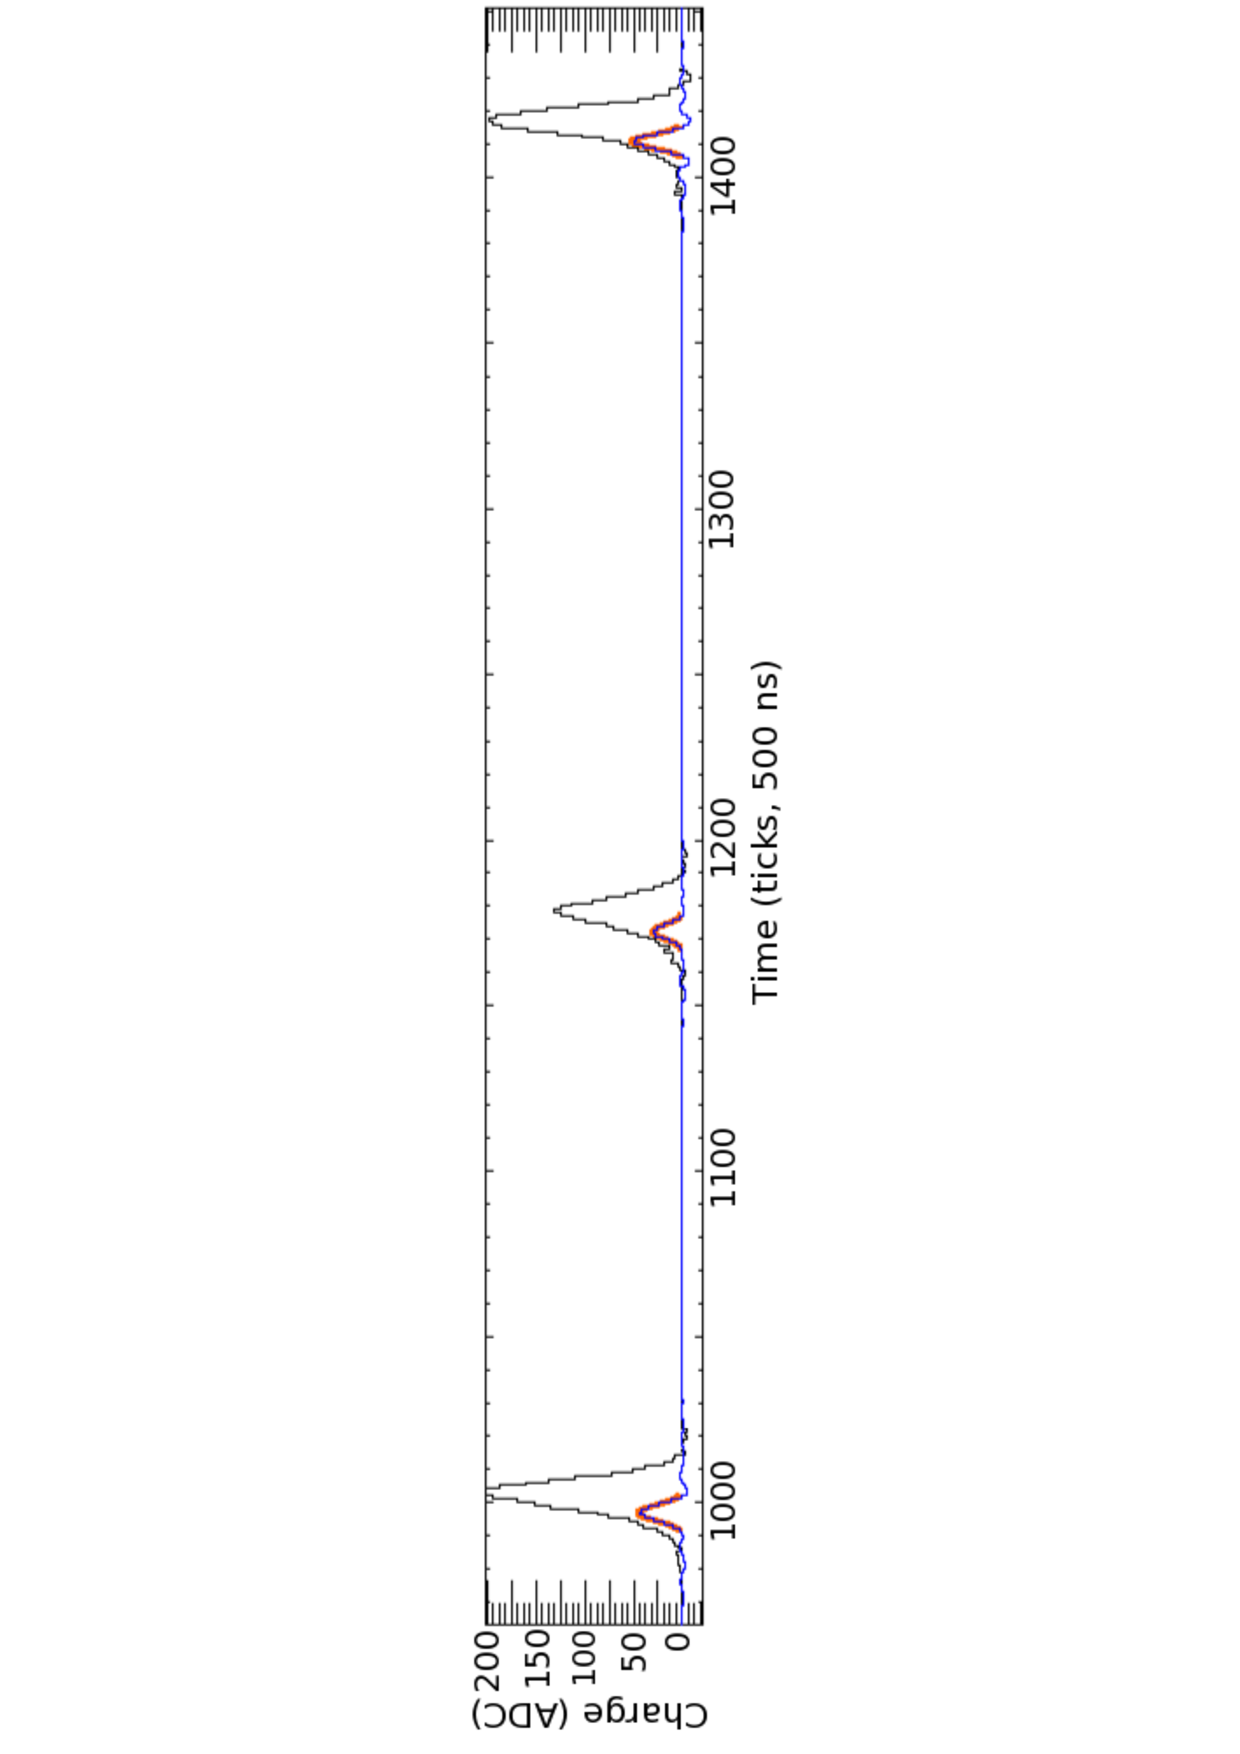
\includegraphics[width=\textwidth]{CollectionPlane}
    \caption{Collection plane depositions.}
  \end{subfigure}
  \begin{subfigure}{0.95\textwidth}
    \centering
    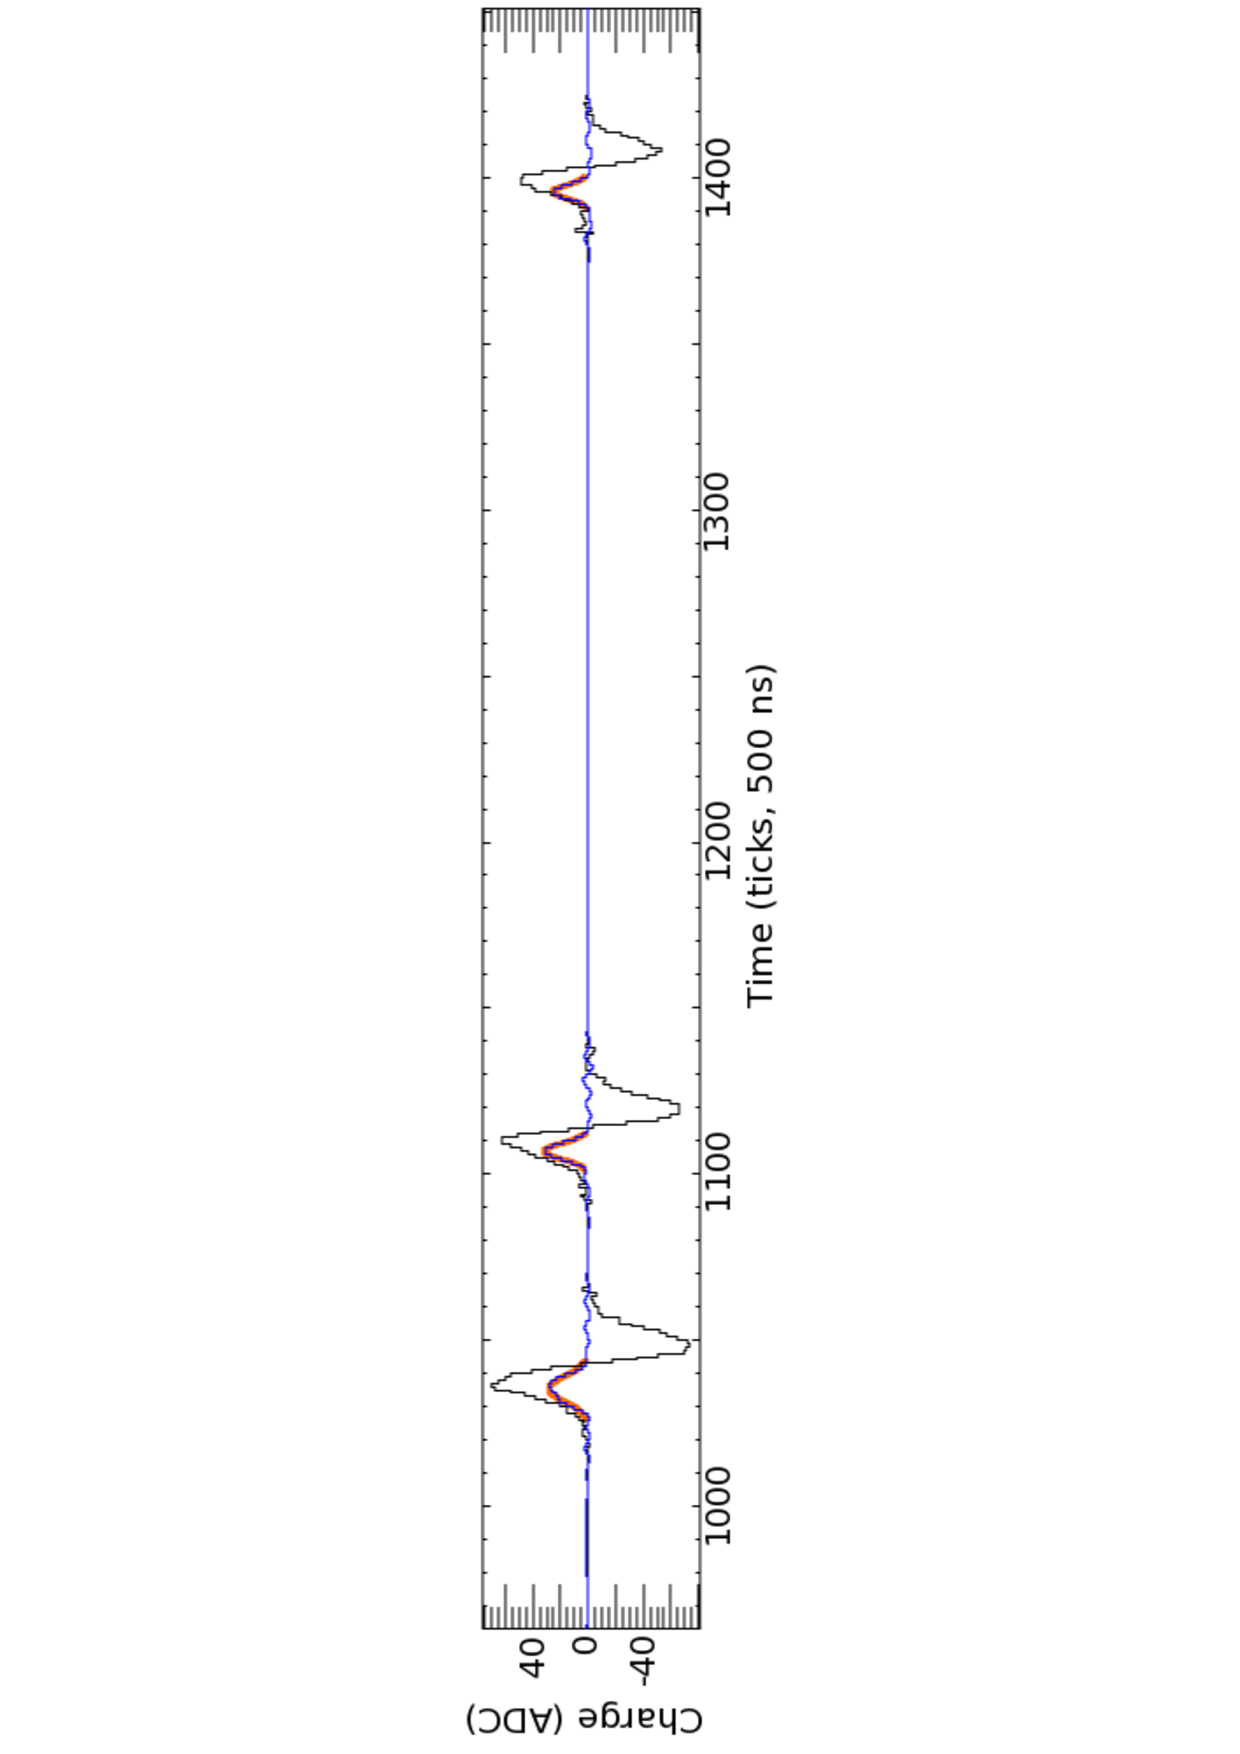
\includegraphics[width=\textwidth]{InductionPlane}
    \caption{Induction plane depositons.}
  \end{subfigure}
  \begin{subfigure}{0.95\textwidth}
    \centering
    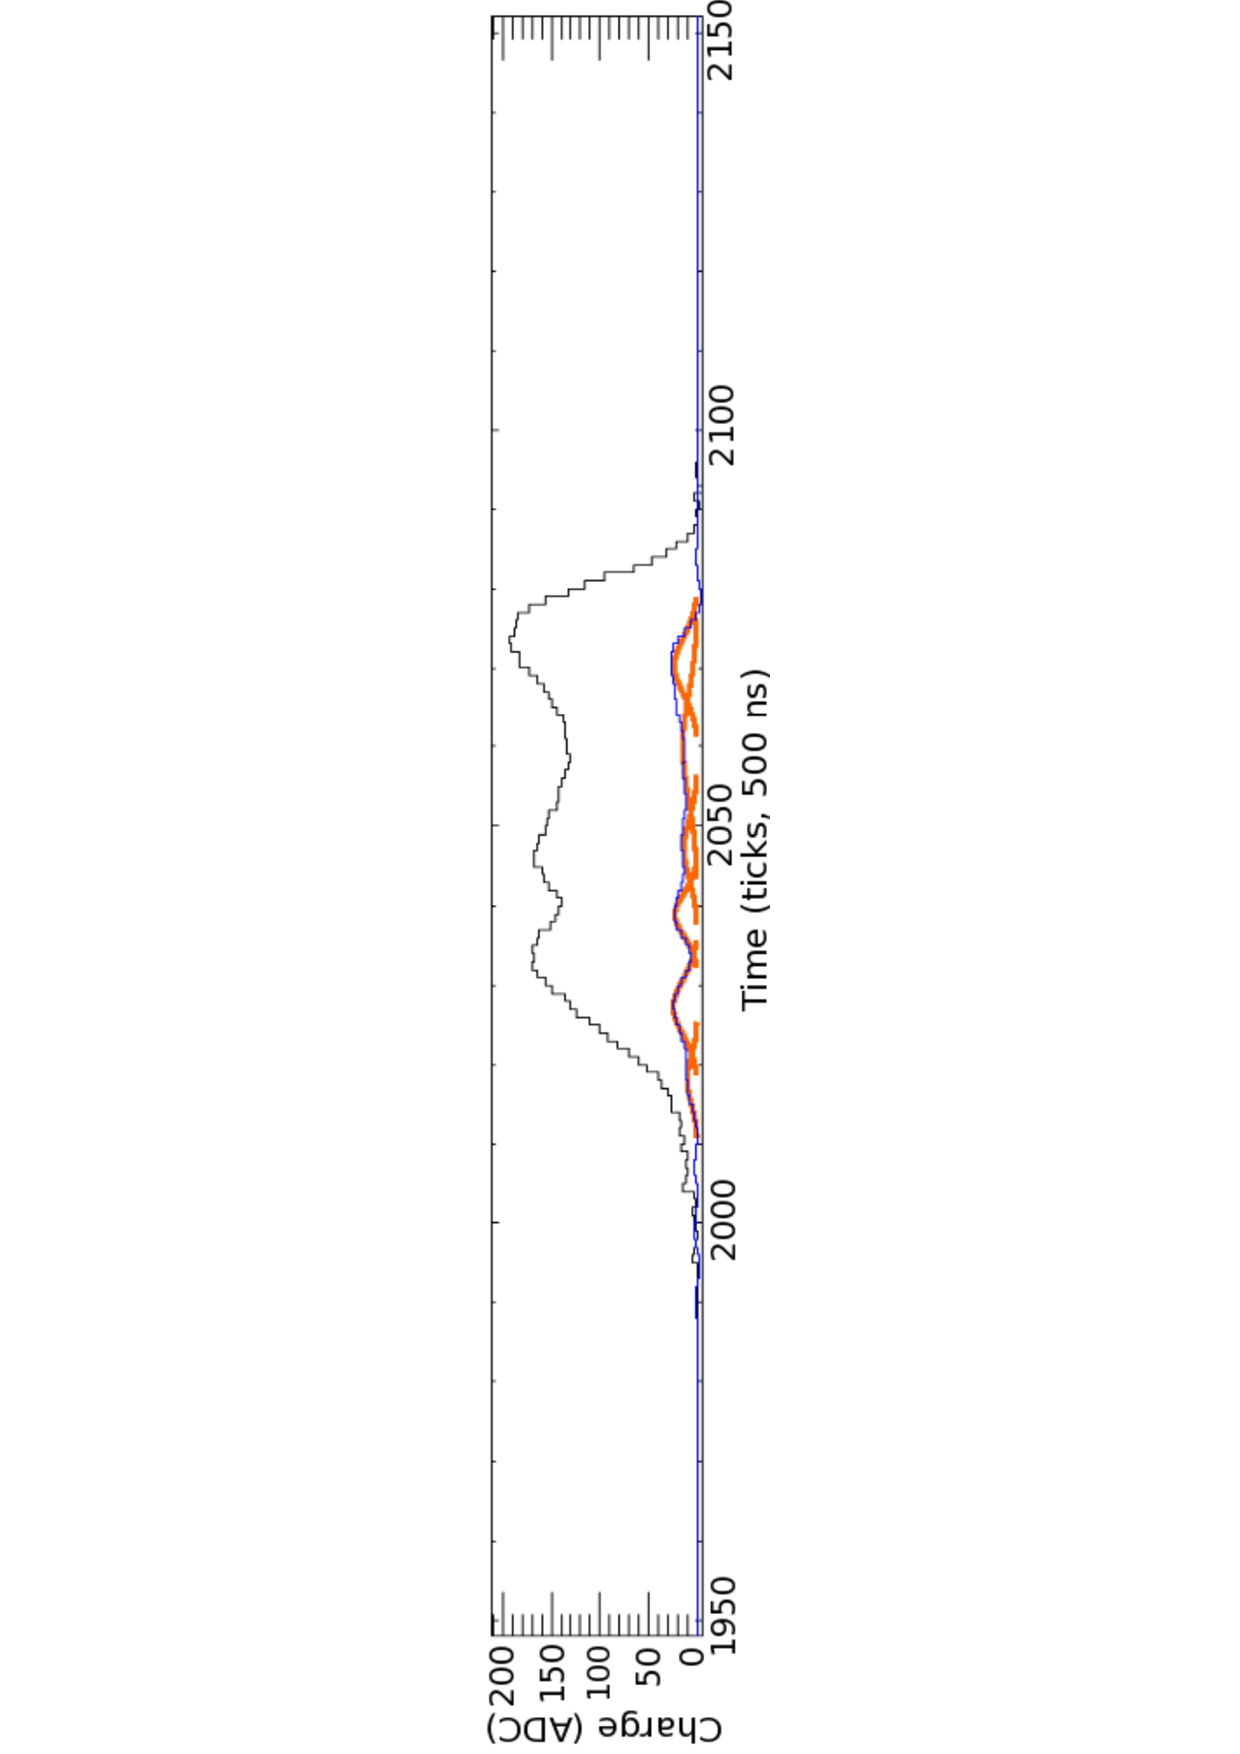
\includegraphics[width=\textwidth]{Complex}
    \caption{A large collection plane deposition over a large period of time.}
  \end{subfigure}
  \caption[Reconstructed hits from a simulated energy deposition]{The raw and deconvoluted signals with reconstructed hits on a single wire for a simulated energy deposition. The plot is shown with increasing charge on the $y$ axis, and increasing time (in ticks) on the $x$ axis. The black line shows the raw signal, the blue line shows the deconvoluted signal and the orange lines show the reconstructed hits.}
  \label{fig:LotsOfHits}
\end{figure}

As noted in Section~\ref{sec:DUNEDetector} and Section~\ref{sec:The35tonDetector} the DUNE FD and the 35 ton both have wrapped wires on the induction planes. A result of this is that the location of where the reconstructed hit occured on an induction wire is ambiguous as a single wire has many wire segments, as shown in Figure~\ref{fig:35tonWireGeom}. An important feature of this ambiguity is that the TPC in which the hit occured cannot be identified unless it is combined with another hit. These ambiguities do not extend to the collection plane wires as they are not wrapped and so consist of only a single wire segment in a single TPC. Hits are combined across the three planes by identifying wire segments on each plane which intersect and have hits at common times. In the traditional reconstruction process only hits that make these so-called 'triple points' are considered dismabiguated, with other hits being identified as noise hits causing them to be discarded. \\

The inclination of the wire planes has to be carefully chosen so as to minise both the number of wires requried and the number of times that wire triplets intersect. It is also important that all wires on a given APA are either read at the top or base of the APA due to the number of APAs required to build a detector of DUNEs scale. The inclination of wires in the 35 ton was 45$^{\circ}$ $\pm$ 0.7$^{\circ}$ meaning that many wire triplets cross twice and some wire pairs cross three times. When wire triplets cross multiple times the triplet which has the smallest distance between the common intersection point and the two-wire intersection points is chosen as the best intersection candidate. The different wire pitches are neccessary so that one of the triple points can be evaluated to be a better candidate, as with a wire pitch of 45$^{\circ}$ both triple points would be equally good fits. The inclination of wires in the FD was chosen to be 36$^{\circ}$ to remove the possibility of multiple intersection points as given the geometry of the APAs multiple intersection points are impossible and so disambiguation is much simpler, but there are more wires on each of the induction planes making it more expensive to instrument. This is shown in Figure~\ref{fig:WirePitches}. \\

\begin{figure}[h]
  \centering
  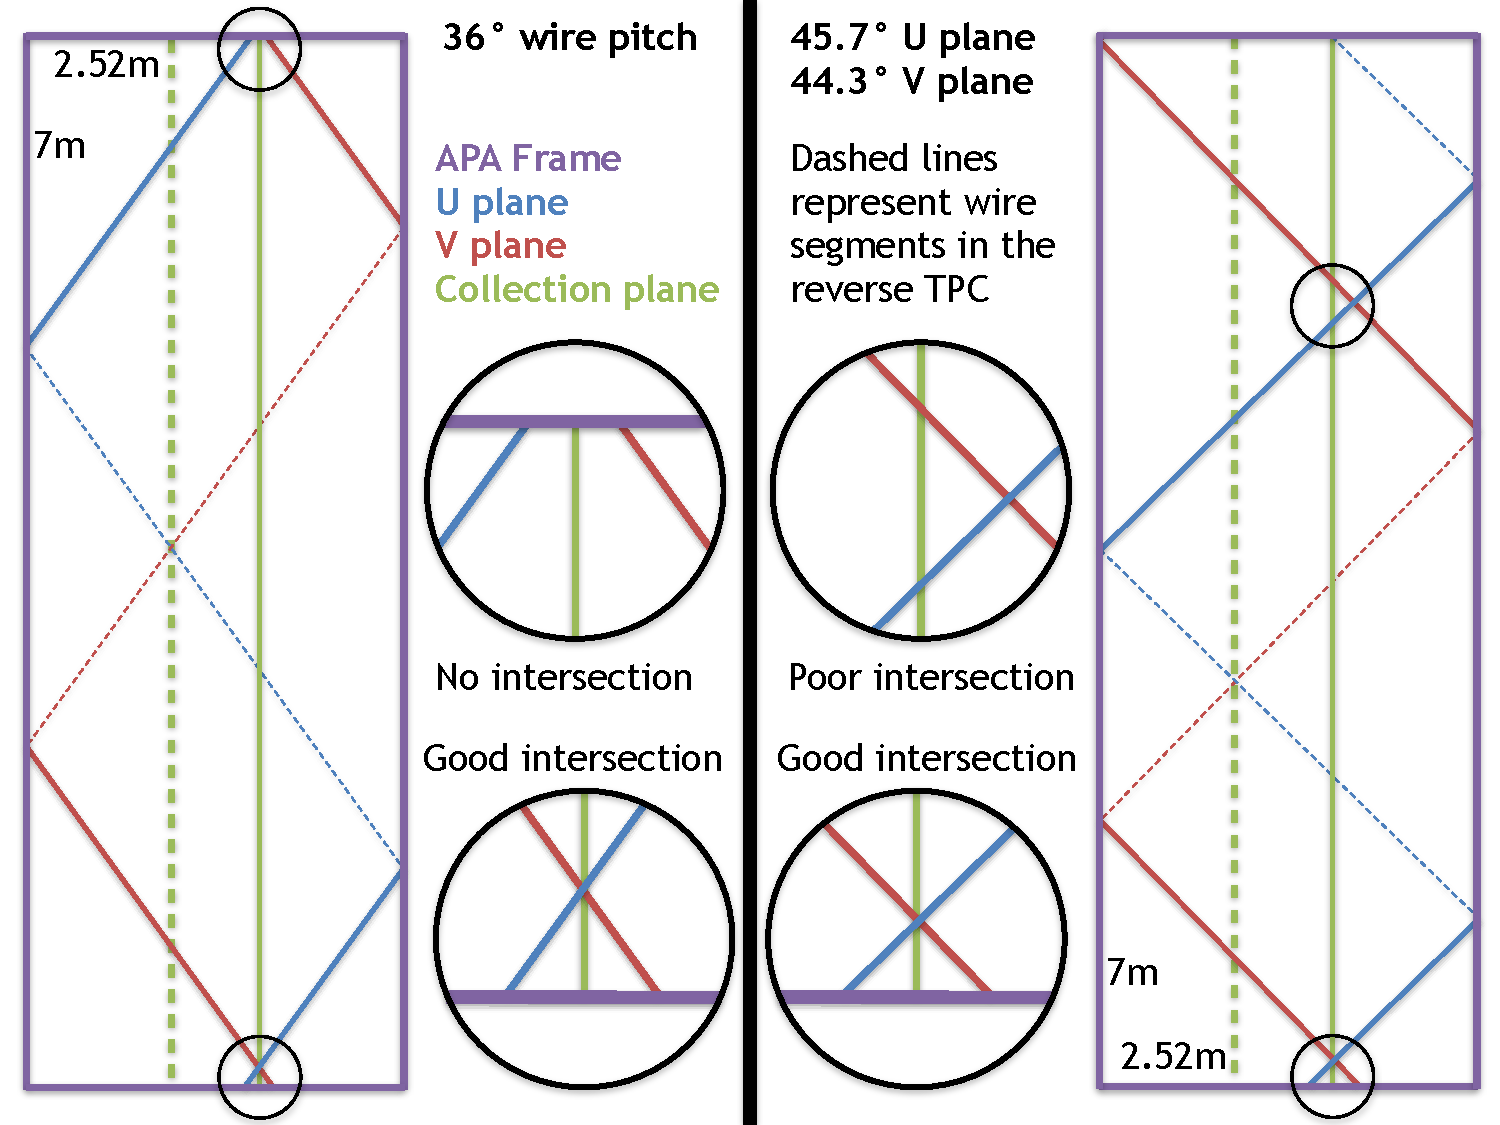
\includegraphics[width=0.85\textwidth]{WireAngleCondition}
  \caption[Performing disambiguation with different wire pitches.]
          {The effect that different wire pitches have on the ability to perform disambiguation in APA with the far detector geometry. The left panel shows a wire pitch of 36$^{\circ}$, which is the reference design for the far detector, whilst the right panel shows wire pitches of 45$^{\circ}$ $\pm$ 0.7$^{\circ}$, as was used in the 35 ton.}
  \label{fig:WirePitches}
\end{figure}

Once the hits have been disambiguated they are combined to make clusters in each of the three planes, before the clusters are merged to make reconstructed tracks or showers. The clustering process is usually performed in wire-tick space on each plane separately with hits from a single physical entitiy being grouped together. It is possible to help seed the start of clusters by using imaging techniques such as a Harris transform, or to identify straight lines by using Hough transforms. As hits from a physical entity are unlikely to remain on a single channel or all come at identical times, clusters are often spread out over many channels for a range of times especially when performing clustering for showers. \\

Once clusters have been identified in each plane they can then be merged into 3-dimensional tracks and showers. The two most common tracking algorithms are PMATrack!!citep{PMATrack}!! and Pandora!!citep{Pandora}!!, and the two most common showering algorithms are EMShower3D!!citep{EMShower3D}!! and EMShower!!citep{EMShower}!!. Once 3D objects have been reconstructed the calorimetric quantities need to be determined, this is often done separately for each plane. Two models exist for calculating $\frac{dE}{dx}$ in LArSoft, Birks model!!citep{BirksModel}!! and a modified box model!!citep{ModBox}!!, though traditionally the later is used. Both models calculate the $\frac{dE}{dx}$ of a hit using the deposited charge ($dQ$) and the track pitch ($dx$) of the hit as well as the conversion of ADC value to number of electrons ($C_{GeV \rightarrow e^{-}}$), the LAr density ($\rho$), the electric field ($E_{field}$) and the tunable electron recombination factors ($Recomb_{X}$). The series of equations used in Birks model is shown in Equation~\ref{eq:Birks}, whilst those used in the modified box are shown in Equation~\ref{eq:ModBox}.

\begin{subequations}\begin{align}
    \frac{dE}{dx} &= \frac{ dQdx_{e} }{ A - B } \label{eq:Birks} \\
    dQdx_{e} &= \frac{ dQ \times C_{lifetime} }{ dx \times C_{ADC \rightarrow e^{-}} } \\
    A &= \frac{ Recomb_{A} }{ C_{GeV \rightarrow e^{-}} } \label{eq:Birks_A}\\
    B &= \frac{ \frac{Recomb_{B}}{\rho} }{ E_{field} \times dQdx_{e} } \label{eq:Birks_B}
\end{align}\end{subequations}

\begin{subequations}\begin{align}
    \frac{dE}{dx} &= \frac{ e^{A} - Recomb_{A} }{ B } \label{eq:ModBox} \\
    A &= B \times C_{GeV \rightarrow e^{-}} \times \frac{dQ}{dx} \label{eq:ModBox_A}\\
    B &= \frac{ Recomb_{B} }{ \rho \times E_{field} } \label{eq:ModBox_B}
\end{align}\end{subequations}
        
When performing calorimetry it is also important that the interaction time is known so that the $x$ positions of hits can be corrected, as they will be reconstructed assuming an interaction time of 0 s. This assumption is made because when using beam events the beam trigger is placed at a time of $T = 0$. An unknown interaction time causes the hit and track positions to be calculated incorrectly, and will also skew the calorimetrics corrections, as recombination is a drift dependant effect.
